\section{SEQUENCE OF PLAY}
\hfill

Each game consists of two Assault Periods, each consisting of eight Battle Turns. At the beginning of every turn, each player chooses a strategy that will affect the battle order adopted by various parts of his army for that turn.

\subsection{The Assault Period}

Each Assault Period consists of eight Battle Turns. At the end of the First Assault Period, the players check to see if the Assault Period is extended (3.3). If not, the armies are reorganized (11.5) and the Second Assault Period begins. The game ends at the conclusion of the Second Assault Period unless one player has previously achieved his victory conditions (12.0).

\subsection{The Battle Turn}

Each Battle Turn consists of an Order Phase, a Norman Player Phase, a Saxon Player Phase and a Turn Record Phase. The player who is active in the phase is called the \textit{phasing player}; the inactive player is called the \textit{non-phasing player}.

ORDER PHASE

At the beginning of every Battle Turn, each player selects a strategy for that turn (4.2). He then consults his Order Table and rolls two dice for each wing or nationality of his army to determine which battle order it will adopt for that turn. Both players can perform this phase simultaneously.

NORMAN PLAYER PHASE

\begin{enumerate}
    \item \textbf{Rally Segment:} The Norman player attampts to rally his disrupted/routed units. Any routed units that fail to rally must immediately move two hexes to the rear.
    \item \textbf{Norman Missile Segment:} Norman missile units can fire at any enemy units within range. Casualties are taken as they occur.
    \item \textbf{Norman Movement Segment:} All unrouted and undisrupted Norman units can move if their order allows.
    \item \textbf{Saxon Reaction Segment:} Non-phasing Saxon units in proper order can move according to the rules governing reaction (5.4).
    \item \textbf{Saxon Missile Segment:} Non-phasing Saxon missile units can fire at any enemy units within range. Only bowman units can fire after taking a reaction move.
    \item \textbf{Melee Segment:} The Norman player melees all Saxon units exerting \textit{zones of control} (5.7) on his units. Casualties are taken immediately, then any units that must retreat must do so.
\end{enumerate}

THE SAXON PLAYER PHASE

The Saxon player repeats 1-6 above, with the Saxon and Norman player reversing roles.

TURN RECORD PHASE

At the end of the Saxon Player Turn, the players advance the Battle Turn Marker on the Turn Record Track. At the end of the First Assault Period, if no decision has been reached, the players reform their armies (see 11.5) and advance the Assault Period Marker on the Assault Period Display, returning the Battle Turn Marker to the beginning of the Turn Record Track. At the end of the second period, the game is over.

\subsection{The Extended Assault Period}

\subsubsection{} The standard Assault Period lasts eight Battle Turns. However, under the following circumstances the Assault Period can be extended:

\begin{enumerate}[label=*]
    \item If more than 50\% of the Norman combat units are on Senlac Hill at the end of the eighth Battle Turn, the period is extended \textit{two} more turns.
    \item If more than 75\% of the Norman combat units are on Senlac Hill at the end of the eighth Battle Turn, the period is extended \textit{three} more turns.
    \item If \textit{all} undisrupted, unrouted Saxons are entirely surrounded by Norman units, Norman zones of control, or the map edge, the period is extended until the Normans win or the encirclement is broken.
\end{enumerate}

Only one of these conditions can be applied at any time; they are mutually exclusive. If there is any question, the Norman player chooses. The Assault Period Marker can be placed on the Turn Record Track to mark the end of the extended period.

\subsubsection{} In an extended period, the following special conditions apply:

\begin{enumerate}[label=*]
    \item The Norman player can reroll any Shield Wall and Hold order he rolls if desired (in this case the Norman player can roll separately for the foot or knight section of a ntionality); and
    \item The Saxon player can reroll any Attack \& Pursue order he rolls if desired.
\end{enumerate}

\subsection{Assault Period Display}

\begin{center}
  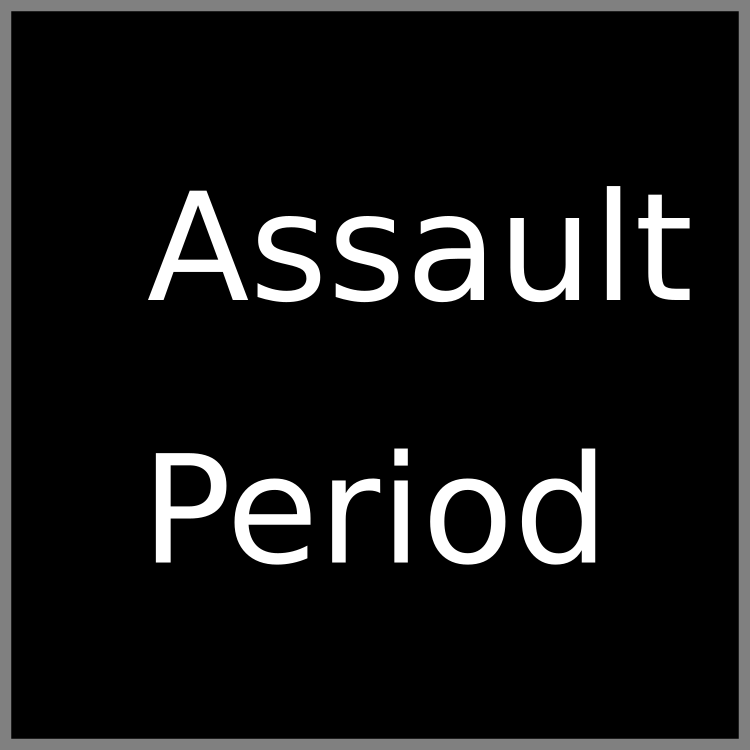
\includegraphics[scale=0.35]{Assault_Period.png}
\end{center}

\subsection{Battle Turn Record Track}

\begin{center}
    
\includegraphics[scale=0.3]{Battle_Turn_Record_Track.png}
\end{center}